\subsection{Two-liquid-phase contact angle method}
\subsubsection{Derivation of Schultz Method}
	%TODO Derive Schultz method for two-liquid-phase}
	
Assuming Young's equation can be applied to a liquid-liquid(bulk phase)-solid ($L_{1}-L_{2}-S$) system, we have the relationship:
\begin{equation}
\label{youngs}
	\gamma_{SL_{2}} = \gamma_{L_{1}L_{2}}\cos\theta_{SL_{1}} + \gamma_{SL_{1}}
\end{equation}

In this way, \gamSV, which is the driving force of spreading the one-liquid-phase method (and causes complete spreading for high-surface energy metal surfaces), is replaced by $ \gamma_{SL_{2}} $, where $\gamma_{SL_{2}} <$ \gamSV. Hence, the contact angle in this system is measurable. 



According to Fowkes \cite{Fowkes1964}, $\gamma_{SL_{1}}$ and $\gamma_{SL_{2}}$ are given by:
\begin{equation} 
\label{gSL1}
	\gamma_{SL_{1}} = \gamma_{S} + \gamma_{L_{1}} - 2(\gamma_{S}^{D}\gamma_{L_{1}}^{D}) - I_{SL_{1}}^{P}
\end{equation}
\begin{equation}
\label{gSL2}
	\gamma_{SL_{2}} = \gamma_{S} + \gamma_{L_{2}} - 2(\gamma_{S}^{D}\gamma_{L_{2}}^{D}) - I_{SL_{2}}^{P}
\end{equation} 
where $\gamma$ and $\gamma^{D}$ are the surface energy and its dispersive component, respectively, and $I_{SL_{1}}^{P}$ is a specific (nondispersive) interaction term that includes all interactions between the solid and the liquid (dipole-dipole, dipole-induced dipole, hydrogen bonds, $\pi$ bonds,...) except London dispersion interactions. 
%TODO Define and understand dispersive vs. polar components of surface energy.
%TODO Define and understand London dispersion forces
Substituting Equations \ref{gSL1} and \ref{gSL2} into \ref{youngs}:

\begin{equation} 
\label{schultz1}
	\gamma_{SL_{1}}-\gamma_{SL_{2}}+\gamma_{L_{1}L_{2}}\cos\theta_{SL_{1}} = 2(\gamma_{S}^{D})^{1/2}  [(\gamma_{L_{1}}^{D})^{1/2}-(\gamma_{L_{2}}^{D})^{1/2}] + I_{SL_{1}}^{P} - I_{SL_{2}}^{P}
\end{equation}

We will be using $L_{1}$ as water, $L_{2}$ as \nalk[s], and $I_{SL_{2}}^{P}$ may be considered equal to zero because the surface free energy of \nalk[s] only consists of the London dispersion term. This is because \nalk[s] only contain C-C and C-H atoms connected by $\sigma$-bonds, with a generic formula of C$_{n}$H$_{2n+2}$. C and H have very similar electronegativities of $\chi_{C}=2.55$ and $\chi_{H}=2.20$, respectively. This shows that all bonds in \nalk[s] are non-polar, hence there are no polar interactions in \nalk[s]. Our final equation is now:

\begin{equation} 
\label{schultz2}
	\gamma_{W}-\gamma_{H}+\gamma_{WH}\cos\theta_{W} = 2(\gamma_{S}^{D})^{1/2}  [(\gamma_{W}^{D})^{1/2}-(\gamma_{H}^{D})^{1/2}] + I_{SW}^{P} 
\end{equation} 

In order to calculate the equilibrium value of \gamSV for a surface, we can interpret Equation \ref{schultz2} as a classic linear function, $y = mx + b$:

\[
\underbracket{\gamma_{W}-\gamma_{H}+\gamma_{WH}\cos\theta_{W}}_{\text{\normalsize{$y$}}} =
\underbracket{2(\gamma_{S}^{D})^{1/2}}_{\text{\normalsize{$m$}}}  
\underbracket{[(\gamma_{W}^{D})^{1/2}-(\gamma_{H}^{D})^{1/2}] }_{\text{\normalsize{$x$}}} + 
\underbracket{I_{SW}^{P}}_{\text{\normalsize{$b$}}} 
\] 
A data set of xy-coordinates will be made by dropping water in an \nalk environment to determine $\gamma_{S}^{D}$ and $I_{SW}^{P} $. $\gamma_{S}^{D} $ will be calculated from the slope of the measured dataset. We can represent the polar interaction by the geometric mean of the polar component of the surface free energy of liquid and solid according to the Equation \ref{Isw} proposed by Owens and Wendt \cite{Owens1969}. The solid surface energy can then be determined from Equation \ref{gamS}:
\begin{equation}
\label{Isw}
	\begin{split}
	I_{SW}^{P} 							& = 2 (\gamma_{S}^{P}\gamma_{L}^{P})^{1/2} \\
	\rightarrow ~ \gamma_{S}^{P}	& = \frac{(I_{SW}^{P})^{2} }{4\gamma_{L}^{P}} 
	\end{split}
\end{equation}
\begin{equation}
\label{gamS}	\gamma_{S} = \gamma_{S}^{D} + \gamma_{S}^{P}	
\end{equation}

Literature values from Schultz et al.\cite{Schultz1977} allow us to use Equation \ref{schultz2} to calculate $\gamma_{S}$:

\begin{table}[h!]
\centering
\caption{Hydrocarbon surface tension and water-hydrocarbon interfacial energy}
\begin{tabular} { |c||c|c|  } %\label{nalkSE}
%	\hline
%	\multicolumn{3}{|c|}{Hydrocarbon surface tension and water-hydrocarbon interfacial energy}\\
	\hline
	\textbf{\nalk[s]}	&\textbf{$\bm{\gamma_{H}}$ (mJ/m$\bm{^{2}}$)}	&\textbf{$\bm{\gamma_{WH}}$ (mJ/m$\bm{^{2}}$)}	\\
	\hline
	hexane		&18.4	&50.1 \\
	\hline
	octane		&21.7	&49.8 \\
	\hline
	decane		&23.8	&51.8 \\
	\hline
	hexadecane	&27.5	&51.3 \\
	\hline
\end{tabular}
\label{knownsurften}
\end{table}
%TODO How are polar and dispersive components of surface tension determined?

Surface energy of muscovite mica will be determined to verify data published in Schultz et al.\cite{Schultz1977,Schultz1992}, and validate the accuracy of the experimental apparatus. 

The following 

\subsubsection{Experimental plan}
\begin{outline}[enumerate]
\1 Make 4 different acrylic glass (Poly(methyl methacrylate), PMMA) boxes for hexane, octane, decane, and hexadecane environments
	\2 Acrylic has high chemical compatibility with \nalk[s] \cite{Thermoscientific}		
	\2 Since most adhesives are stored in \nalk[s] (also commonly used as industrial strength degreasers), PMMA boxes must be chemically welded together by a solvent at room temperature to keep the liquid environment contained. 
\1 Polish single-crystal samples and EBSD them to check surface orientation. After the main sample surface orientation is discovered, the sample can be cut to obtain \hkl(001), \hkl(110), and \hkl(111) facets. Each sample is then polished again for EBSD measurement. 
\1 Mount samples if flat samples cannot be achieved, and initiate two-liquid-phase method
	\2 Measure static contact angles
		\3 These are expected to either completely wet the surface in less than one second or return contact angles with a large margin of error due to the variability between receding and advancing angles. 
		\3 One option is to use a high speed camera to capture the split second spreading of water on the metal surface. This could potentially capture an advancing contact angle before the droplet spreads completely. An advancing \ca can approximate the Young \ca since it is another minimum in the Gibbs free energy curve.
	\2 Measure advancing and receding contact angles (CAs) for contact angle hysteresis (CAH)
		\3 CAH will give accuracy of equilibrium CA on flat surface. 
	\2 Use advancing CA for calculations
		\3 For ideal-like flat surfaces, the advancing contact angle can be approximated as the Young contact angle. The accuracy of this can be determined by measuring the contact angle hysteresis on a given surface. The greater the CAH, the less reliable the approximation. 
\1 Pattern surfaces with transparency paper $\gtrsim$40 $\mu$m since this is the lower limit of transparency paper. A rough surface will increase the water contact angle, and the known roughness will allow calculation of a Young contact angle to be used in surface energy calculation. 

\begin{figure}[h]
	\centering
		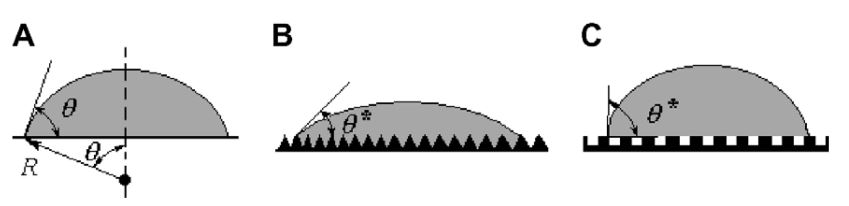
\includegraphics[width=\linewidth]{young_cassie_wenzel}
	\caption{Schemes of different wetting regimes. A – flat substrate; B – rough substrate, the Wenzel regime; C – rough substrate with air trapped under the drop, the Cassie–Baxter regime.\cite{Whyman2008}}
	\label{fig:young_cassie_wenzel}
\end{figure}

	\2 The assumption of this patterned surface is that the Cassie-Baxter or Wenzel contact angle is the most stable contact angle, and the Young contact angle can be approximated using the Cassie-Baxter and Wenzel equations. This contact angle will be suitable for the of metal surface energy that will be calculated from Equation \ref{schultz2}.
		\3 There seems to be controversy in literature on whether the equilibrium contact angle calculated in Cassie and Wenzel equations can be used as the Young \ca.\cite{Attension2015,Marmur2009b,Bracco2013}
		\3 The Cassie-Baxter contact angle is an equilibrium contact angle as proven by Johnson and Dettre using thermodynamic principles.\cite{Johnson1964}
		\3 The most stable contact angle on a rough surface is either the Wenzel or Cassie angle, IF the size of the drop is two to three orders of magnitude larger than the typical scale of roughness.\cite{Meiron2004} %TODO: read the paper cited, about sufficient drop size vs. roughness
	\2 Preliminary two-liquid-phase method experiments on muscovite mica showed quick and complete wetting of water on pristine mica surfaces cleaved in decane and hexadecane, contradictory to published results.\cite{Schultz1992} When mica samples were removed from the decane environment, they were wiped clean with KimWipes and further cleaned with acetone. When the samples were returned to the decane environment, a droplet wet the surface with an observable \ca. When this process was repeated in hexadecane, the observed \ca increased as observed in Schultz et al.\cite{Schultz1992} 
	
	This observable \ca is a result of roughening the surface, but because the trend of increasing \ca persists, I hypothesize that an induced roughness on isotropic metal surfaces could show increasing \ca[s] with increasing \nalk chain lengths. These induced roughnesses will be known, and using Wenzel\cite{Wenzel1936,Wenzel1949a} and Cassie\cite{Cassie1944} methods for calculating equilibrium \ca[s] and, resultantly, the orientation-dependent Galfenol surface energy. 
		
	\2 Per conversation with Dave Shahin, an experienced student in patterning surfaces, an array of roughnesses can be made on a single sample to test roughness effects on surface energy measurements of single crystal Galfenol and Alfenol. 
		\3 There is a criteria for determining if the calculated contact angle on a rough surface is in Wenzel and Cassie-Baxter modes. 
	
\1 Redo two-liquid-phase experiment for patterned surface
	\2 Calculate the Cassie and Wenzel mode equilibrium CA
		\3 Expecting Cassie mode because the patterned channels will ideally be completely filled with hydrocarbon/\nalk liquid, thus \underline{repelling} the water droplet on the surface. This is due to the immiscibility of polar (distilled water) and non-polar (\nalk) solvents. 
	\2 \textbf{Is there a difference from one patterned orientation to another?} This will show if the patterning (induced roughness) will have a large impact on the CA and, as a result, \underline{Surface Energy}. 
		\3 If we have a defined roughness for {100}, {110}, and {111} samples
\end{outline}

%\subsection{Induced roughness for Wenzel and Cassie modes}

\subsection{DFT measurements from collaborator}
\subsubsection{Cassie-Baxter or Wenzel mode}
\textbf{Can Dr. Ruqian Wu simulate a sessile drop in a two-liquid-phase experiment on a patterned surface?} This can tell us if we can expect Cassie of Wenzel mode of water drop in hydrocarbon/\nalk environment. 

\subsubsection{Two compositions of single crystal Galfenol}
Dr. Wu has assigned a student to working on a difference in \fegacomp surface energy where $x =$ 19 and 25.